\documentclass[11pt]{article}
\usepackage{lscape}
\usepackage{amsmath,amssymb}
\usepackage{amsthm}
\usepackage{float}
\usepackage{booktabs}
\usepackage{graphicx}
\usepackage{comment}
\usepackage{bm}
\usepackage{gensymb}
\allowdisplaybreaks[4]
\usepackage{geometry}
\geometry{margin=1in}
\usepackage{setspace}
\usepackage{siunitx}
\usepackage{enumitem}
\usepackage{dsfont}

\usepackage{graphics}


\usepackage[utf8x]{inputenc}
\usepackage{bm}

\usepackage{hyperref}
\hypersetup{
    colorlinks=true,
    citecolor = blue,
    linkcolor=blue,
    filecolor=magenta,           
    urlcolor=cyan,
}


\theoremstyle{plain}
\newtheorem{thm}{Theorem}[section]
\newtheorem{lem}{Lemma}
\newtheorem{conjecture}{Conjecture}
\newtheorem{prop}{Proposition}
\newtheorem{pro}{Property}
\newtheorem{cor}{Corollary}
\newtheorem{ass}{Assumption}

\theoremstyle{definition}
\newtheorem{defn}{Definition}
\newtheorem{exmp}{Example}
\newtheorem{rmk}{Remark}

\usepackage{algpseudocode,algorithm}
\algnewcommand\algorithmicinput{\textbf{Input:}}
\algnewcommand\algorithmicoutput{\textbf{Output:}}
\algnewcommand\INPUT{\item[\algorithmicinput]}
\algnewcommand\OUTPUT{\item[\algorithmicoutput]}



\usepackage[labelfont=bf]{caption}

\setcounter{table}{1}
\usepackage{multirow}
\usepackage{tabularx}

\def\fixme#1#2{\textbf{[FIXME (#1): #2]}}

 

\newcommand*{\KeepStyleUnderBrace}[1]{%f
  \mathop{%
    \mathchoice
    {\underbrace{\displaystyle#1}}%
    {\underbrace{\textstyle#1}}%
    {\underbrace{\scriptstyle#1}}%
    {\underbrace{\scriptscriptstyle#1}}%
  }\limits
}
\usepackage{mathtools}
\mathtoolsset{showonlyrefs=true}


\usepackage{hyperref}
\hypersetup{colorlinks=true}
\usepackage[parfill]{parskip}
\usepackage{bm}
\onehalfspacing


\usepackage{stmaryrd}
\newtheorem{Example}{Example}  
\newtheorem{Definition}{Definition}
\newtheorem{Theorem}{Theorem}
\newtheorem{Assumption}{Assumption}
\newtheorem{Proposition}{Proposition}
\newtheorem{Conjecture}{Conjecture}

\newtheorem{Lemma}{Lemma}
\newtheorem{Remark}{Remark}
\newtheorem{Corollary}{Corollary}


\input macros.tex
\def\rank{\textup{Trank}}

\def\Mat{\textup{Mat}}

%\usepackage[mathscr]{eucal}
\usepackage{mathrsfs}
\def\calif{\large\mathscr{F}}
\def\caliT{\large\mathscr{T}}
\def\tL{\large\mathscr{L}}

\begin{document}
\begin{center}
{\bf \Large Infinitely smooth single index model for tensors}\\
Miaoyan Wang, Nov 09, 2021\\
\end{center}


\section{Model}
We use $f^{(\ell)}(x)$ to denote the $\ell$-th derivative of $f$, evaluated at $x$. 
\begin{defn}[Analytic function class] Let $C>0$ be a positive constant. The analytic function class $\calif(C)$ on $[-1,1]$ is defined as the set of functions $f\colon [-1,1]\to \mathbb{R}$ whose derivatives satisfy
%A function $f\colon[-1,1]\to\mathbb{R}$ is called analytic if there exists a constant $C>0$ such that
\[
\sup_{x\in[-1,1]}|f^{(\ell)}(x)|\leq C^{\ell+1}\ell! \quad \text{for all }\ell\in\mathbb{N}_{+}.
\]
Equivalently, $f$ is infinitely differentiable and its Taylor expansion around any point in its domain converges to the function. 
%We use $\tH(C)$ to denote the collection of analytic functions defined over $[-1,1]$.  
\end{defn}

%For any $\alpha\geq 0$, we call the function $f\colon [-1,1]\to\mathbb{R}$ is Holder-$\alpha$ smooth if
%\[
%\sup_{x\in\tX}|f^{\ell}(x)|\leq {\color{red}a^{\ell}\ell!}\quad \text{and}\quad {1\over \ell !}|f^{(\ell)}(x)-f^{(\ell)}(y)| \leq L\mnormSize{}{x-y}^{\alpha-\lfloor \alpha\rfloor}.
%\]
%Single index matrix family
%\begin{align}
%\tP(d,\alpha,s,L)&=\left\{\mTheta\colon \mTheta=f(\mX\mY^T) \text{ for some matrices }\mX, \mY \in\mathbb{R}^{d\times s} \text{ and function } f\in \tH(\alpha,L), \notag \right.\\ 
%& \left. \quad \norm{\mX}_{2\to\infty}=\norm{\mY}_{2\to\infty}=1 \right\}.
%\end{align}
%Single index tensor family
%\begin{align}
%\tP(d,s,C)&=\left\{\Theta\colon \Theta=f(\tB) \text{ for some dim-$d$ rank-$s$ tensor with } \mnormSize{}{\tB}=1 \text{ and function }f\in\tH(C)\right\}.
%\end{align}
%Note that the scalar of $\tB$ is absorbed into $C$. 

A higher-order tensor $\tT$ can be unfolded into a matrix. We now introduce several quantities that controls the complexity of matrix unfolding. We use $\Mat(\tT)$ to denote the matrix unfolding. We use $\rank(\cdot)$ and $\lambda(\tT)$ the rank and spectral norm of the matrix $\Mat(\tT)$, 
\[
\rank(\tT):=\text{rank}(\Mat(\tT)), \quad  \lambda(\tT):=\snormSize{}{\Mat(\tT)}.
\]
The following family consists of $d$-dimensional order-$m$ tensor with Tucker rank bounded by $r$. 
\begin{defn}[Low-rank tensor class] The family of $d$-dimensional rank-$s$ tensor $\caliT(d,s,m)$ is defined as the set of tensors with Tucker rank bounded by $r$:
\[
\caliT(d,s,m)=\{\tT\in (\mathbb{R}^{d})^{\otimes m}\colon \rank(\tT)\leq s \text{ and } \lambda(\tT)\leq 1\}
\]
\end{defn}
Equivalently, the tensor in class $\caliT(d,s,m)$ admits the rank-$s$ Tucker decomposition:
\[
\tT=\tC\times_1\mX\times\cdots\times_k \mX.
\]
where $\tC\in\mathbb{R}^{s\times \cdots \times s}$ is core tensor and $\mX$ are factor matrices with orthornormal columns. The condition $\lambda(\tT)\leq 1$ is imposed without loss of generality. The scale between $\tT$ and the $f$ is undetermined; the tensor $f(\tT)=f'(\tT')$ are the same by setting $\tT'=c\tT$ and $f'=f/c$. 
We also note that, the rank-$s$ CP tensor is automatically included in $\caliT(d,s,m)$. 
%\[
%\tB\over 
%\]
%with $\norm{\mM_i}_{2,\infty}\leq 1$ and $\lambda_{\max}(\tM(\tC))\leq \sqrt{s}$. 


Now, we are ready to describe the main model. Let $\tY$ be the data tensor. We propose the following observation model
\begin{equation}\label{eq:index}
\tY=f(\tT)+\tE, \quad \text{ for some unknown } \tT\in\caliT(d,s,m) \text{ and }f\in\calif(C),
\end{equation}
where we assume the noise tensor $\tE$ consists of i.i.d.\ entries with zero-mean and sub-Gaussian parameter $\sigma^2$. We call~\eqref{eq:index} the \emph{single index tensor model}. The name of single index model comes from the observation that 
\[
\mathbb{E}\left[\tY(\omega)|\tX(\omega)\right]=f(\langle \tT,\  \tX(\omega)\rangle), \quad \text{for all }\omega\in[d]^m,
\]
where, for every index $\omega$, the predictor $\tX(\omega)\in(\mathbb{R}^d)^{\otimes m}$ is a dummy-variable tensor with 1 at the $\omega$-th position, and zero everywhere else. 
Note that the signal tensor $f(\tT)$ is often high rank. Our goal is to address the following two questions:
\begin{itemize}
\item What are the \emph{statistical} and \emph{computational} limits for signal estimation in single index model?
\item Are there any intrinsic distinctions for matrices $m=2$ vs.\ tensors $m\geq 3$ for high-rank estimation based on model~\eqref{eq:index}?
\end{itemize}



\section{Smooth single index models are of log-rank}
Let $\tT\in \caliT(d,s,m)$, and $\tT^{\circ \ell}$ be the tensor of the same size, with entrywise polynomial transformation $a\to a^\ell$. We have the following rank bound.
\begin{prop}[Monomial tensor] For every tensor $\tT\in\caliT(d,s,m)$ and every natural number $\ell\in\mathbb{N}_{+}$
\[
\rank(\tT^{\circ \ell})\leq {\ell+s-1 \choose s-1}.
\]
\end{prop}
This proposition shows the polynomial rank growth with respect to $\ell$. The exponent depends on the original rank $s$, which is assumed small. When $s=1$, then $\rank(\tT^{\circ \ell})=1$ for all $\ell\in\mathbb{N}_{+}$. The bound is nontrivial when $\ell \leq d$. In fact, later we will set $\ell \lesssim \log d$. 

\begin{figure}
\centering
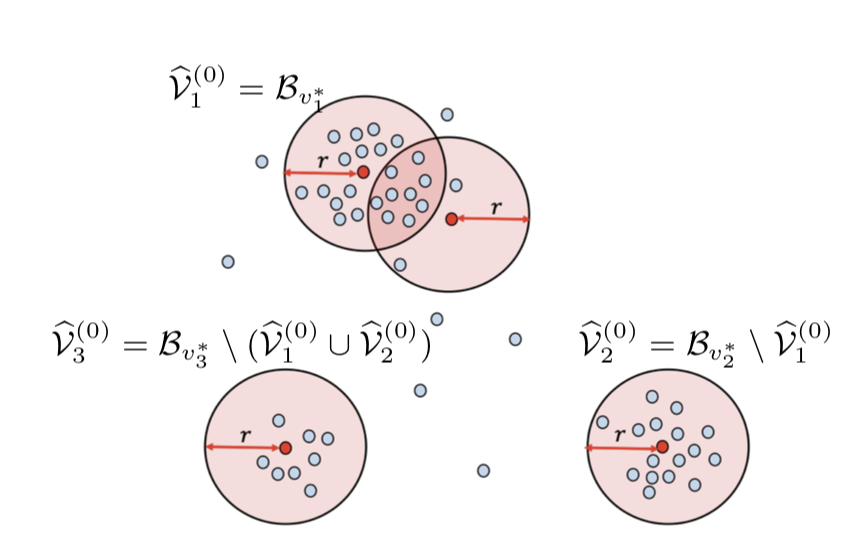
\includegraphics[width=.5\textwidth]{illustrate.png}
\end{figure}

\begin{prop}[Uniform approximation for single index tensor]\label{prop:approximation} Consider $\tT\in\caliT(d,s,m)$ and $f\in\calif(C)$.  There exists a set of basis tensors $\{\tB_{\ell,k}\colon (k,\ell)\in[d]\times\mathbb{N}\}$, such that, for every number of pieces $k\in[d]$ and degree $\ell\in\mathbb{N}$, we have
\[
\mnormSize{}{f(\tT)-\tB_{k,\ell}}\leq C\left( {k\over sm}\right)^{-(\ell+1)} \quad \text{and}\quad \rank(\tB_{k,\ell})\leq k^{s}\ell^s.
\]
\end{prop}


The following is the key property of single index matrix by taking $k\gtrsim \Omega(sm)$ and $\ell=r^{1/s}k^{-1}$ in Proposition~\ref{prop:approximation}.
\begin{thm}[Dimension-free approximation error]\label{thm:approximation} Consider a single index tensor $\Theta=f(\tT)$, where $\tT\in \caliT(d,s,m)$ and $f\in\calif(C)$. For every rank $r\in\mathbb{N}_{+}$,  we have
\[
{1\over d^m}\FnormSize{}{\Theta-\textup{Proj}_r(\Theta)}^2 \lesssim C^2\exp\left(-{r^{1/s}\over sm}\right).
\]
The bound is uniform over $\tT\in\caliT(d,s,m)$ and $f\in\calif(C)$. 
\end{thm}

\begin{cor}[Nice smooth tensor model is of $\log$ rank] For any fixed $\varepsilon>0$, we have
\[
\rank_{\varepsilon}(\Theta):=\min\{\rank(\tA)\colon \mnormSize{}{\tA-\Theta}\leq \varepsilon\}\lesssim \log^s d.
\]
\end{cor}


\section{Estimation algorithm}


\subsection{Non-convex double spectral algorithm}

\begin{thm}[Polynomial algorithm] low-rank approximation is substantially better. 
\begin{align}
\tR(\hat \mTheta,\mTheta)\leq
\begin{cases}
r^{m}+d^{m/2}r+d^mr^{-2\alpha}& r^{-2\alpha}\leq d^{-(m-1)},\\
\min(d^{{-{m\over 2}+{(m-\alpha-1)m\over 2\alpha}}},1) &  \alpha\leq {(m-1)^2\over m},\ r\asymp \min(d^{(m-1)/2\alpha},d)\\
d^{-{{m\over 2}+{m-1\over 2\alpha}}}& \alpha\geq {(m-1)^2\over m}, \ r\asymp  d^{m-1\over 2\alpha}\leq d^{m\over 2(m-1)}\\
d^{-{m\over 2}}\log d & \alpha=\infty, \ r\asymp \log d
\end{cases}
\end{align}
\end{thm}

\begin{thm}[Minimax optimality for tensors] 
Order-$m$ with known design (bottleneck: truncate at $d^{-(m-1)}$ with unknown design)
\begin{align}
\tR(\hat \mTheta,\mTheta)\leq
\begin{cases}
d^{-{2\alpha m \over m+2\alpha}} & \alpha\leq {m(m-1)\over 2}\\
d^{-{(m-1)}}\log d& \alpha\geq {m(m-1)\over 2}
\end{cases}
\end{align}
\end{thm}


\bibliography{yourbibfile}

\newpage
\appendix
\section{Proof of Proposition 1}
\begin{proof}
By definition $\tT\in\caliT(d,s,m)$, $\rank(\Mat(\tT))\leq r$. Therefore, there exists matrix SVD such that
\[
\Mat(\tT)=\sum_{i\in[s]} \lambda_i\ma_i\otimes \mb_i,
\]
where $\ma_i\in\mathbb{R}^d$, $\mb\in\mathbb{R}^{d^{m-1}}$, and $\lambda_1\geq \cdots \lambda_s\geq 0$. By definition
\begin{align}\label{eq:svd}
\Mat(\tT^{\circ \ell})&=\left[\Mat(\tT)\right]^{\circ \ell}=\left(\sum_{i\in[s]}\lambda_i\ma_i\otimes \mb_i\right)^{\circ \ell}\\
&=\sum_{\substack{\kappa_1+\cdots+\kappa_s=\ell,\\ (\kappa_1,\ldots,\kappa_s)\in\mathbb{N}^s_{+}}}\lambda^{\kappa_1}_1\cdots\lambda^{\kappa_s}_s(\ma^{\circ \kappa_1}_1\circ \cdots \circ \ma^{\circ \kappa_s}_s)\otimes(\mb^{\circ \kappa_1}_1\circ \cdots \circ \mb^{\circ \kappa_s}_s).
\end{align}
Here $(\ma^{\circ \kappa_1}_1\circ \cdots \circ \ma^{\circ \kappa_s}_s) \in\mathbb{R}^{d}$ and $(\mb^{\circ \kappa_1}_1\circ \cdots \circ \mb^{\circ \kappa_s}_s)\in\mathbb{R}^{d-1}$. Now notice that by counting argument, 
\[
\#\{(\kappa_1,\ldots,\kappa_s) \in \mathbb{N}_{+}^{s} \colon \kappa_1+\cdots+\kappa_s=\ell\} = {\ell+s-1 \choose s-1}.
\]
Therefore, the summation~\eqref{eq:svd} consists of no more than ${\ell+s-1 \choose s-1}$ rank-1 terms. We conclude that
\[
\rank(\tT^{\circ \ell})=\text{rank}(\Mat(\tT^{\circ \ell}))\leq  {\ell+s-1 \choose s-1}.
\]
\end{proof}
\section{Proof of Lemma 2}
\begin{lem} we have
\[
\mnormSize{}{f(\tT)-\tB_{k,\ell}}\leq {\max_{|\eta|\leq 1}|f^{(\ell+1)}|(\eta)\over (\ell+1)!}\mnormSize{}{(\tT-\tO)^{\circ {\ell+1}}}\leq \left({k\over sm}\right)^{-(\ell+1)}. 
\]
\end{lem}
Note that the covering number of $s$-dimensional bounded set $\tX$ is $\tN(1/k, \tX, \mnormSize{}{\cdot})\leq k^s$. Let $\tE_k$ denote the corresponding covering set. Then,  $\tE_k$ satisfies 
\begin{enumerate} 
\item $|\tE_k| \leq k^s$;
\item For every $\Delta \in\tE_k$, we have
\[
 \max_{\mx_i,\mx_j\in \Delta}\mnormSize{}{\mx_i-\mx_j}\lesssim {1\over k}.
\]
\item $\Delta \cap \Delta'=\emptyset$ for all $\Delta\neq \Delta'\in\tE_k$.
\end{enumerate}
We label the center of the covering set by $\{\mo_1,\ldots,\mo_{k^s}\} \subset\{\mx_1,\ldots,\mx_d\}$. We use $z\colon [d]\to[k^s]$ to denote the membership of rows of $\mX$
\[
z(i)=\argmin_{j\in[k^s]}\mnormSize{}{\mx_i - \mo_j}, \quad\text{such that}\quad \mnormSize{}{\mx_i-\mo_{z(i)}}\leq {1\over k}.
\]
We define a block matrix $\tO\in(\mathbb{R}^{d})^{\otimes m}$ with entries
\[
\tO(i_1,\ldots,i_m)=\tC\times_1\mo_{z(i_1)}\times_2\cdots\times_m \mo_{z(i_m)} 
\]
Therefore
\[
\mnormSize{}{\tT-\tO}\leq \max_{(i_1,\ldots,i_m)\in[d]^m} |\tC\times_1 \mx_{i_1}\times_2\cdots \times_m \mx_{i_m}-\tC\times_1 \mo_{z(i_1)}\times_2\cdots \times_m \mo_{z(i_m)}|\lesssim mk^{-1}s^{1/2}.
\]
Define 
\[
\tB_{k,\ell}:=f^{(1)}(\tO)\circ (\tT-\tO)+{f^{(2)}(\tO)\over 2}\circ (\tT-\tO)^{\circ 2}+\cdots {f^{(\ell)}(\tO)\over \ell!} \circ (\tT-\tO)^{\circ \ell}.
\]
The membership partition $[d]^m$ into $k^{sm}$ blocks. We use $[d]^m=\cup_{n=1}^{k^{sm}}\Delta_n$ to denote these blocks. Within each block, the tensor $\tO$ takes the same value, 
\begin{align}
\tB_{k,\ell}(\omega)&=\KeepStyleUnderBrace{(a_{0,\Delta}+a_{1,\Delta}\tT+a_{2,\Delta}\tT^{\circ 2}+\cdots a_{\ell,\Delta} \tT^{\circ \ell})}_{:=\tI}\mathds{1}\{\omega\in \Delta \}.
\end{align}
%By the definition of $\tB$
%\[
%\Mat(\tB_{k,\ell})(i_1,i_{-1})=\sum_{j\in[k^s]} (a_{0,j,i_{-1}}+a_{1,j,i_{-1}}\Mat(\tT)+a_{2,j,i_{-1}}\Mat(\tT^{\circ 2})+\cdots a_{\ell,j,i_{-1}} \Mat(\tT^{\circ \ell}))\mathds{1}\{i_1\in\Delta_j\}.
%\]
Because there are $k^{s}$ blocks along mode 1, we conclude that
\[
\rank(\tB_{k,\ell})\leq k^{s} \sum_{n=1}^\ell{n+s-1 \choose s-1} \leq k^{s}(\ell+s-1)^s.
\]


\begin{thm}[Dimension-free approximation] Let $\Theta\in\tP(d,s,L)$. For every rank $r\in\mathbb{N}_{+}$,  
\[
{1\over d^m}\FnormSize{}{\Theta,\ \text{Proj}_r(\Theta)}^2\lesssim L^2\exp(-c_0r^{1/s}).
\]
\end{thm}
\begin{proof}
Let $k=\Omega(2a)$ and $\ell=r^{1/s}k^{-1}$. Then
\[
\mnormSize{}{\Theta-\tA_{k,\ell}}\leq L 2^{-\ell}\ell^{ms} \lesssim L2^{-\ell}\asymp L\exp(-r^{1/s})
\]
\end{proof}

\end{document}
